%%%%%%%%%%%%%%%%%%%%%%%%%%%%%%%%%%%%%%%%%
% University/School Laboratory Report
% LaTeX Template
% Version 3.1 (25/3/14)
%
% This template has been downloaded from:
% http://www.LaTeXTemplates.com
%
% Original author:
% Linux and Unix Users Group at Virginia Tech Wiki 
% (https://vtluug.org/wiki/Example_LaTeX_chem_lab_report)
%
% License:
% CC BY-NC-SA 3.0 (http://creativecommons.org/licenses/by-nc-sa/3.0/)
%
%%%%%%%%%%%%%%%%%%%%%%%%%%%%%%%%%%%%%%%%%

%----------------------------------------------------------------------------------------
%	PACKAGES AND DOCUMENT CONFIGURATIONS
%----------------------------------------------------------------------------------------

\documentclass{article}

\usepackage[version=3]{mhchem} % Package for chemical equation typesetting
%\usepackage{siunitx} % Provides the \SI{}{} and \si{} command for typesetting SI units
\usepackage{graphicx} % Required for the inclusion of images
\usepackage{natbib} % Required to change bibliography style to APA
\usepackage{amsmath} % Required for some math elements 
\usepackage{hyperref}
 \usepackage{pdflscape}
\usepackage[a4paper,margin=0.5in]{geometry}
\setlength\parindent{0pt} % Removes all indentation from paragraphs

\renewcommand{\labelenumi}{\alph{enumi}.} % Make numbering in the enumerate environment by letter rather than number (e.g. section 6)

%\usepackage{times} % Uncomment to use the Times New Roman font

%----------------------------------------------------------------------------------------
%	DOCUMENT INFORMATION
%----------------------------------------------------------------------------------------

\title{Gate Detection} % Title

\author{Philipp \textsc{Duernay}} % Author name

\date{\today} % Date for the report

\begin{document}
\maketitle
% If you wish to include an abstract, uncomment the lines below
% \begin{abstract}
% Abstract text
% \end{abstract}

%----------------------------------------------------------------------------------------
%	SECTION 1
%----------------------------------------------------------------------------------------

\section{Recap}
In the last meeting from 18.07.2018 several next steps were defined:
\begin{itemize}
	\item Investigate performance with respect to bounding boxes
	\item Investigate bounding box accuracy
\end{itemize}

\section{IoU}

Fig. \ref{fig:iou} shows detections at different IoU values. An IoU with 0.4 accepts detections that are quite off, 0.6 seems reasonable.


\begin{figure}[htbp]
	\centering
	\begin{minipage}{0.3\linewidth}
		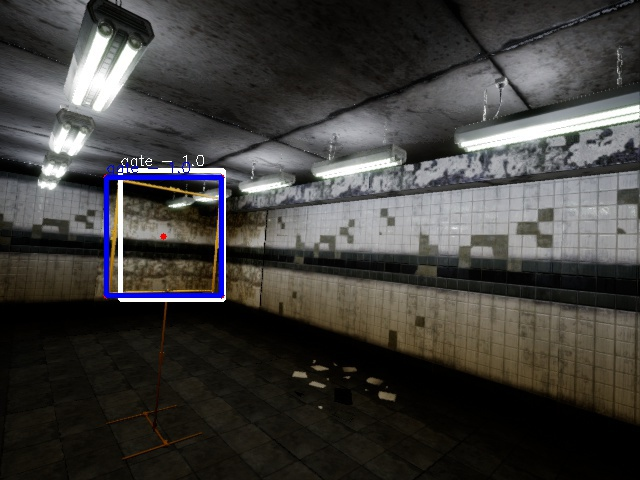
\includegraphics[width=\linewidth]{0000-04.jpg}
	\end{minipage}
	\hfill
	\begin{minipage}{0.3\linewidth}
		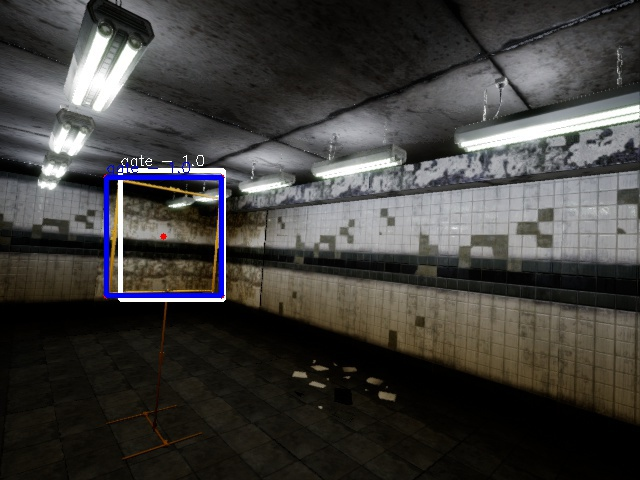
\includegraphics[width=\linewidth]{0000-06.jpg}
	\end{minipage}
	\hfill
	\begin{minipage}{0.3\linewidth}
		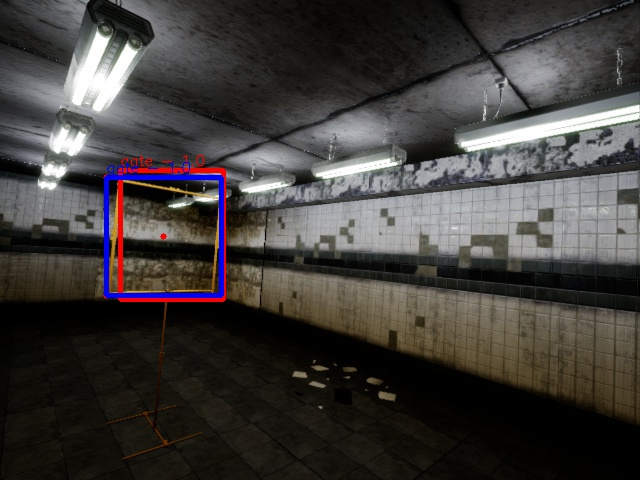
\includegraphics[width=\linewidth]{0000-08.jpg}
	\end{minipage}
	
	\begin{minipage}{0.3\linewidth}
		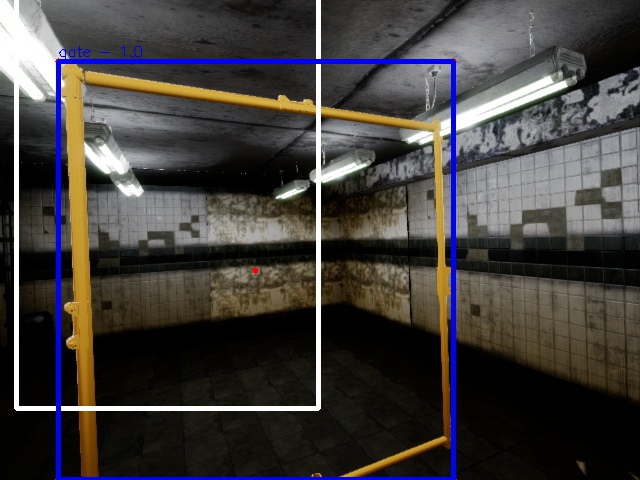
\includegraphics[width=\linewidth]{0021-04.jpg}
	\end{minipage}
	\hfill
	\begin{minipage}{0.3\linewidth}
		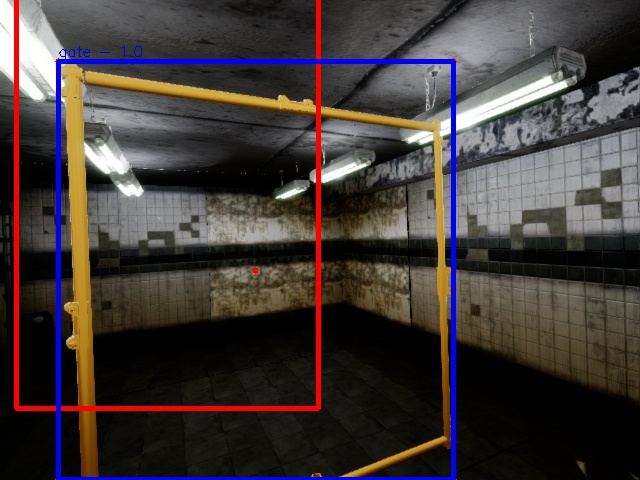
\includegraphics[width=\linewidth]{0021-06.jpg}
	\end{minipage}
	\hfill
	\begin{minipage}{0.3\linewidth}
		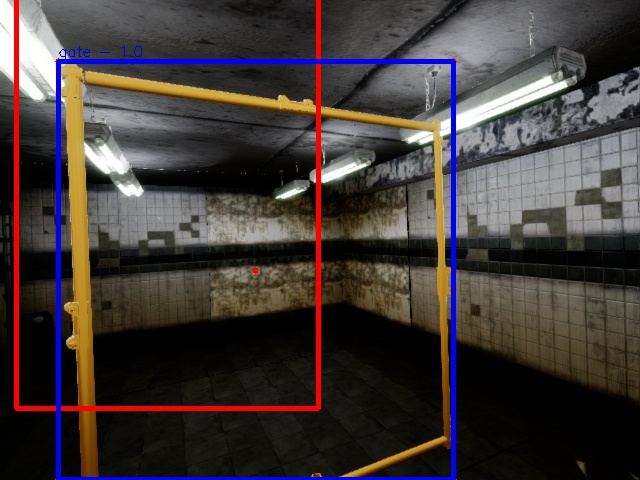
\includegraphics[width=\linewidth]{0021-08.jpg}
	\end{minipage}
	\caption{Two example images at different IoU thresholds with ground truth in blue, true positive in white, false positive in red. From left to right IoU=0.4;0.6;0.8}
	\label{fig:iou}
\end{figure}

\section{Experiment - Receptive Field}

\paragraph{Hypothesis:} The receptive field is crucial for detecting large gates, hence a network with a larger receptive field should perform better on large gates.

\paragraph{Experiment:} Several networks are trained with similar 9-layer architecture a part from the last layer. In the last layer kernel width and height are increased stepwise.

\paragraph{Results:} Results are displayed in Fig. \ref{fig:box_size}. We see what we expected to some extent. While the performance for small gates does not change with the receptive field, the performance for larger gates improves. However, for very large gates this does not hold anymore. A model with small receptive field performs better than the other models.

\paragraph{Conclusion:} The receptive field is important to take into account, as the models perform better the more context they see. However, for large gates it does not solve the problem. 

\begin{figure}[htbp]
	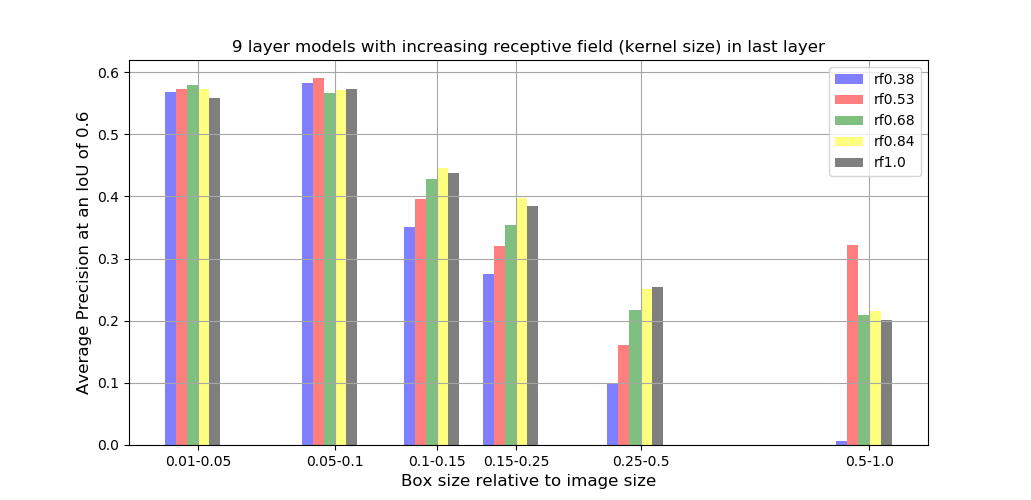
\includegraphics[width=\linewidth]{box_size_rf_06}
	\caption{Average Precision for different box sizes on a test set of 1000 images.}
	\label{fig:box_size}
\end{figure}

\section{Some Images}

Fig. \ref{fig:examples} and following shows different gate sizes. We see how there are much more occlusions when going closer to the gate. Hence, the loss in performance could also be caused by this.


\begin{figure}[htbp]
	\centering
	\begin{minipage}{0.3\linewidth}
		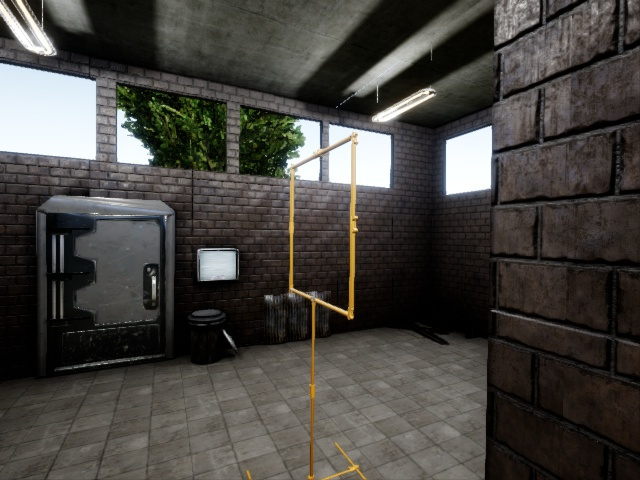
\includegraphics[width=\linewidth]{size_examples/001-005 (1).jpg}
	\end{minipage}
	\hfill
	\begin{minipage}{0.3\linewidth}
		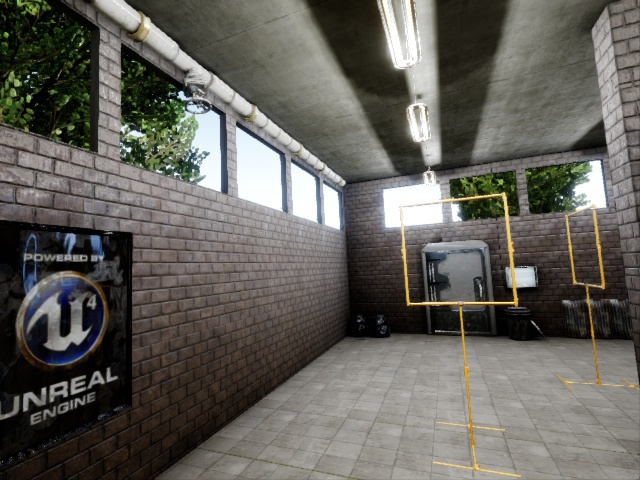
\includegraphics[width=\linewidth]{size_examples/001-005 (2).jpg}
	\end{minipage}
	\hfill
	\begin{minipage}{0.3\linewidth}
		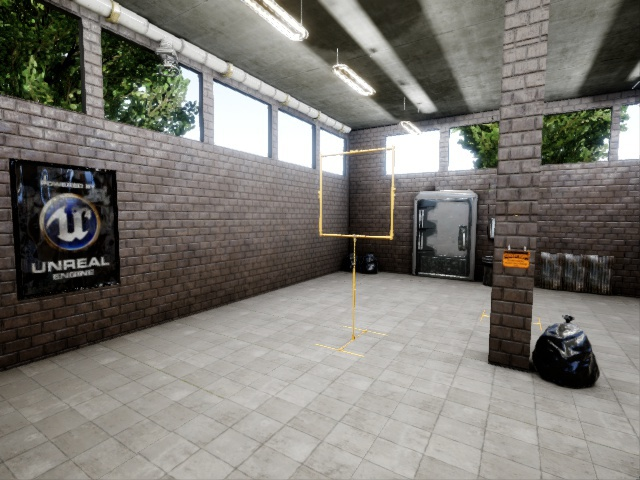
\includegraphics[width=\linewidth]{size_examples/001-005 (6).jpg}
	\end{minipage}
	\caption{Examples for image sizes 0.0-0.05}
	\label{fig:examples}
\end{figure}
\begin{figure}[htbp]	
	\begin{minipage}{0.3\linewidth}
		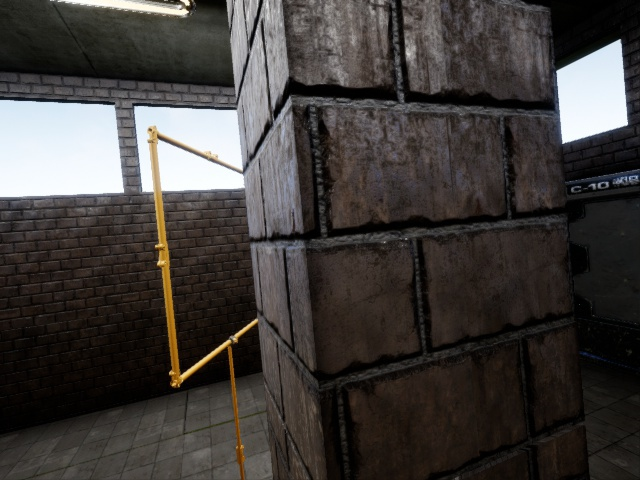
\includegraphics[width=\linewidth]{size_examples/005-01 (1).jpg}
	\end{minipage}
	\hfill
	\begin{minipage}{0.3\linewidth}
		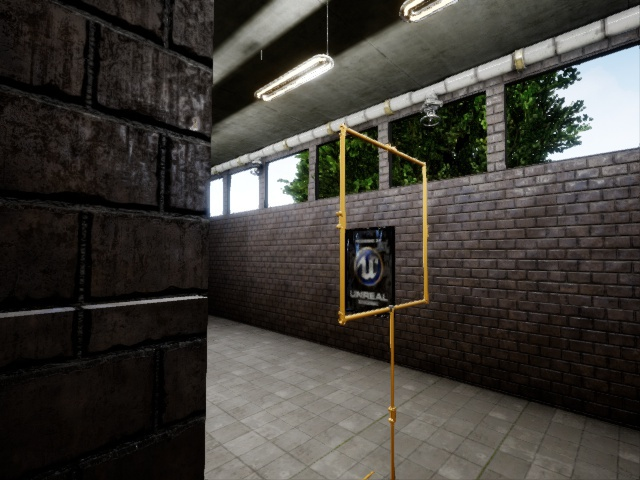
\includegraphics[width=\linewidth]{size_examples/005-01 (8).jpg}
	\end{minipage}
	\hfill
	\begin{minipage}{0.3\linewidth}
		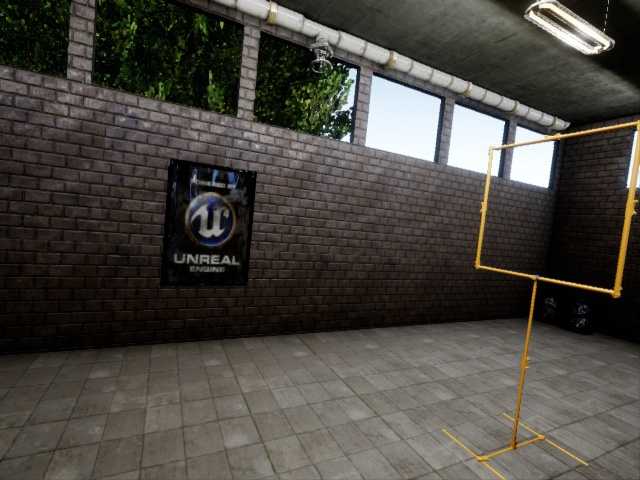
\includegraphics[width=\linewidth]{size_examples/005-01 (7).jpg}
	\end{minipage}
	\caption{Examples for image sizes 0.05-0.1}
\end{figure}
\begin{figure}[htbp]
	\begin{minipage}{0.3\linewidth}
	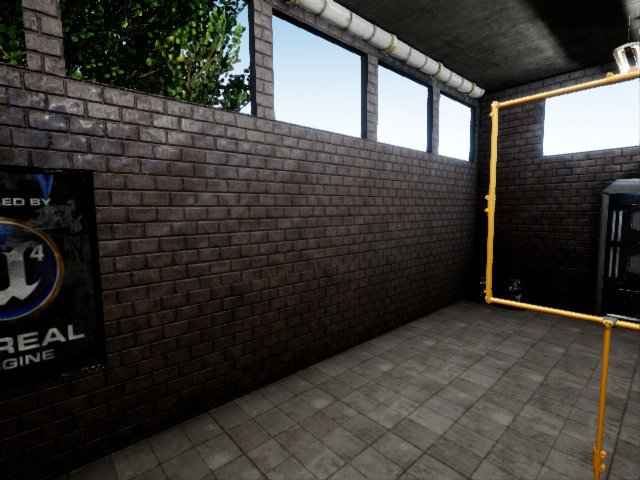
\includegraphics[width=\linewidth]{size_examples/01-015 (1).jpg}
\end{minipage}
\hfill
\begin{minipage}{0.3\linewidth}
	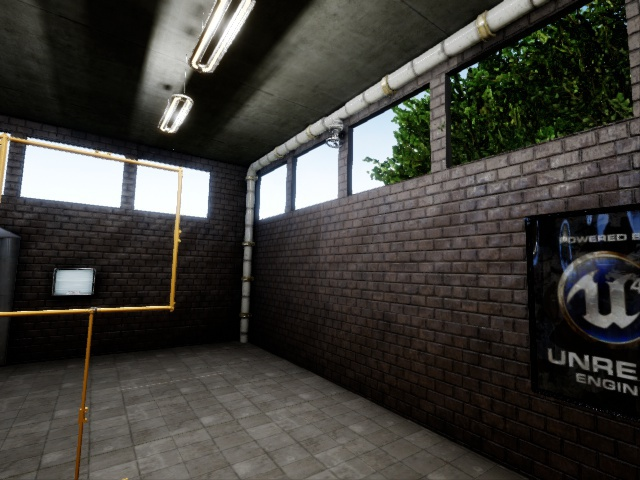
\includegraphics[width=\linewidth]{size_examples/01-015 (9).jpg}
\end{minipage}
\hfill
\begin{minipage}{0.3\linewidth}
	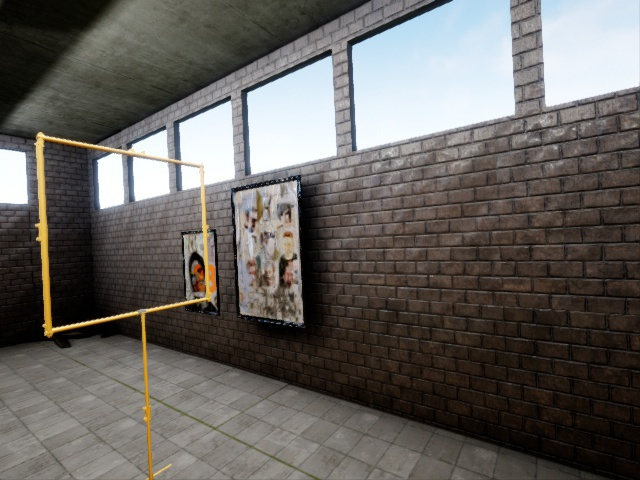
\includegraphics[width=\linewidth]{size_examples/01-015 (7).jpg}
\end{minipage}
	\caption{Examples for image sizes 0.1-0.15}
\end{figure}
\begin{figure}[htbp]
	\begin{minipage}{0.3\linewidth}
	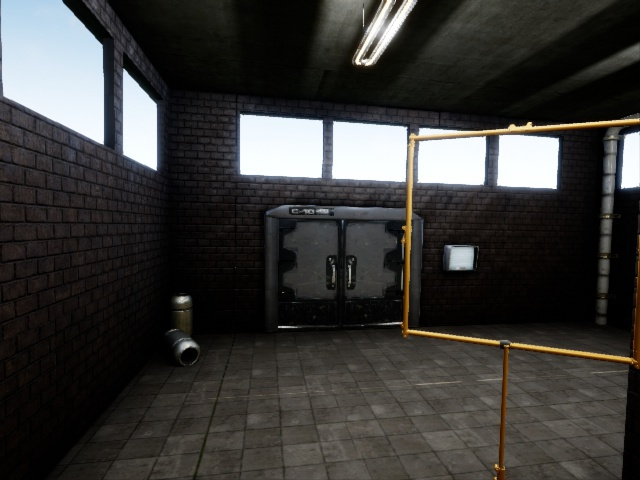
\includegraphics[width=\linewidth]{size_examples/015-025 (2).jpg}
\end{minipage}
\hfill
\begin{minipage}{0.3\linewidth}
	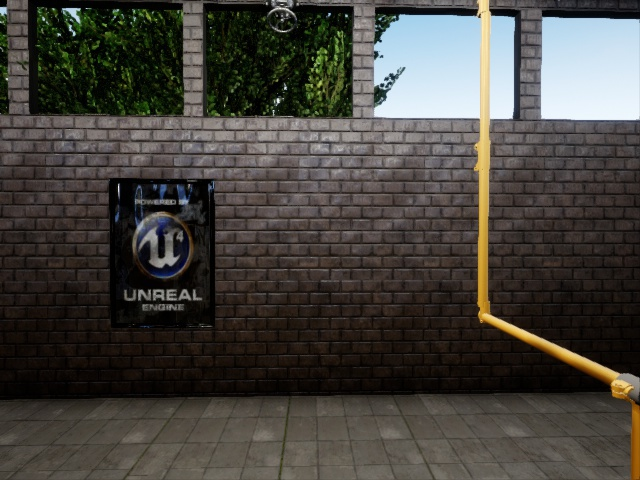
\includegraphics[width=\linewidth]{size_examples/015-025 (3).jpg}
\end{minipage}
\hfill
\begin{minipage}{0.3\linewidth}
	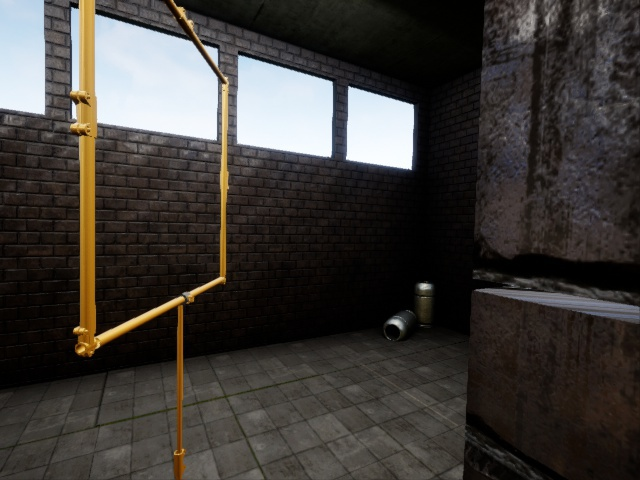
\includegraphics[width=\linewidth]{size_examples/015-025 (7).jpg}
\end{minipage}
	\caption{Examples for image sizes 0.15-0.25}
\end{figure}
\begin{figure}[htbp]
	\begin{minipage}{0.3\linewidth}
	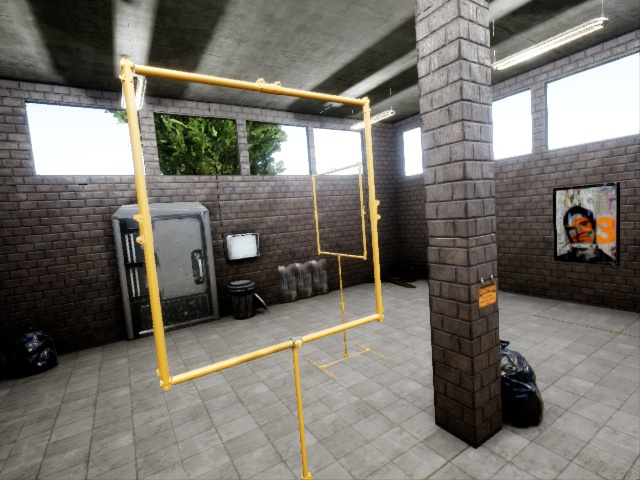
\includegraphics[width=\linewidth]{size_examples/025-05 (1).jpg}
\end{minipage}
\hfill
\begin{minipage}{0.3\linewidth}
	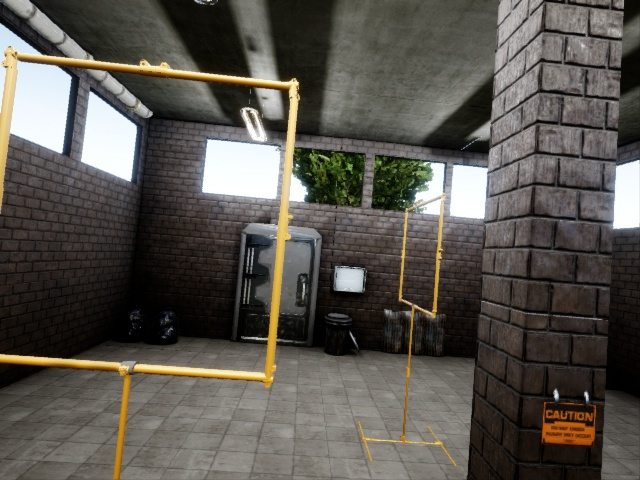
\includegraphics[width=\linewidth]{size_examples/025-05 (9).jpg}
\end{minipage}
\hfill
\begin{minipage}{0.3\linewidth}
	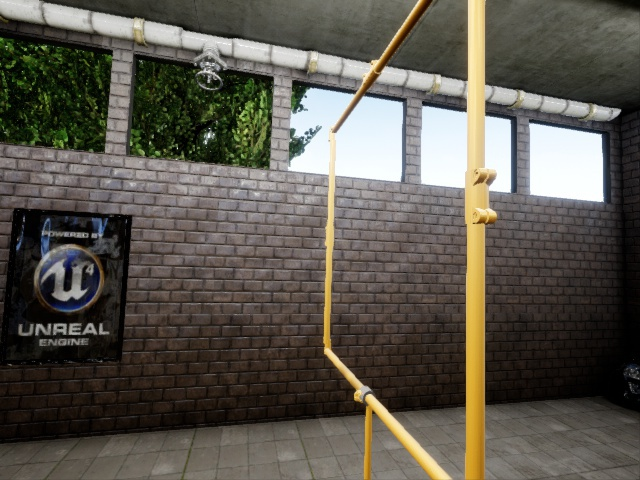
\includegraphics[width=\linewidth]{size_examples/025-05 (7).jpg}
\end{minipage}
	\caption{Examples for image sizes 0.25-0.5}
\end{figure}
\begin{figure}[htbp]
	\begin{minipage}{0.3\linewidth}
	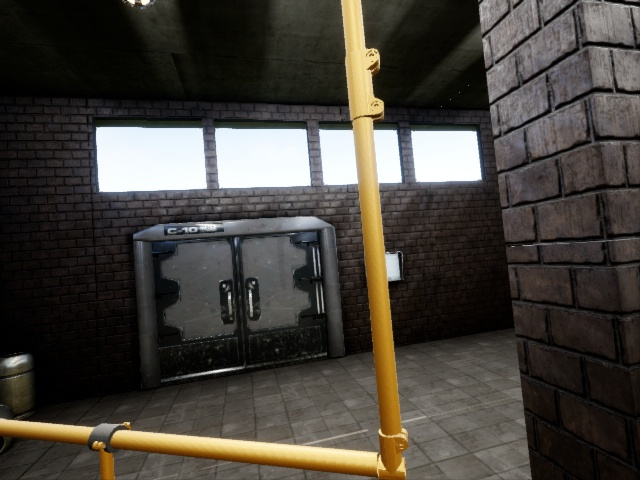
\includegraphics[width=\linewidth]{size_examples/05-10 (1).jpg}
\end{minipage}
\hfill
\begin{minipage}{0.3\linewidth}
	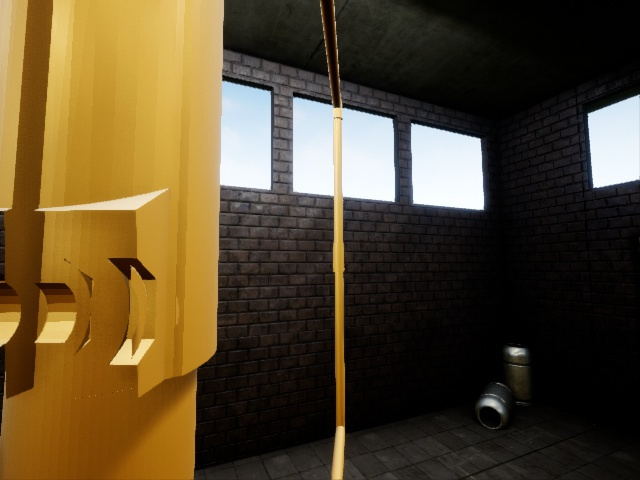
\includegraphics[width=\linewidth]{size_examples/05-10 (10).jpg}
\end{minipage}
\hfill
\begin{minipage}{0.3\linewidth}
	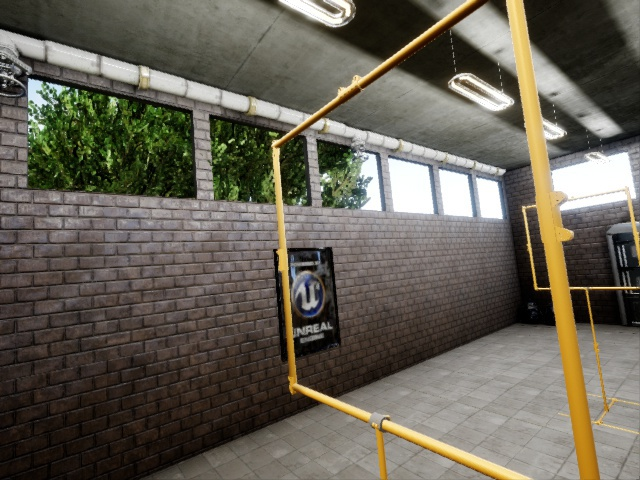
\includegraphics[width=\linewidth]{size_examples/05-10 (7).jpg}
\end{minipage}
	\caption{Examples for image sizes 0.5-1.0}
\end{figure}
\newpage
\section{Experiment - Model}

\paragraph{Hypothesis I:} The first few layers detect all the shapes while the higher layers just "collect" the responses from the image to detect larger gates. A network without the final 4 layers should also be able to at least detect the smaller gates.
\paragraph{Experiment:} Train a network with 5 layers and see performance.
\paragraph{Results:} Results are displayed in Fig. \ref{fig:model}. We see how the small gates can still be detected well. No performance loss at gate sizes of 0.05-0.1. The small performance loss for gates of size 0.01-0.05 can be explained by the reduced resolution.


\paragraph{Hypothesis II:} The final "image" in the network is of size 13,13. Potentially predicting with smaller grid/ larger scale can improve performance while reducing computation.
\paragraph{Experiment:} Train a network with 9 layers but instead of downsampling the image to 13x13 as before we downsample to 7x7 and predict for each cell.
\paragraph{Results:} Results are displayed in Fig. \ref{fig:model}. We see how this model performs much better at larger gates while loosing performance for smaller gates.

\paragraph{Conclusion:} The information in the final grid seems to be related to the object scale. A smaller grid seems to work better for large gates and the other way around.
 
A network that predicts at multiple grid sizes should work well for small and larger boxes. E.g. One could add a prediction layer after layer 5 at a grid size of (13,13) then sample down further to (7,7) and (3,3) and add further prediction layers. This even saves computations as the deeper images get smaller and smaller.


\begin{figure}[htbp]
	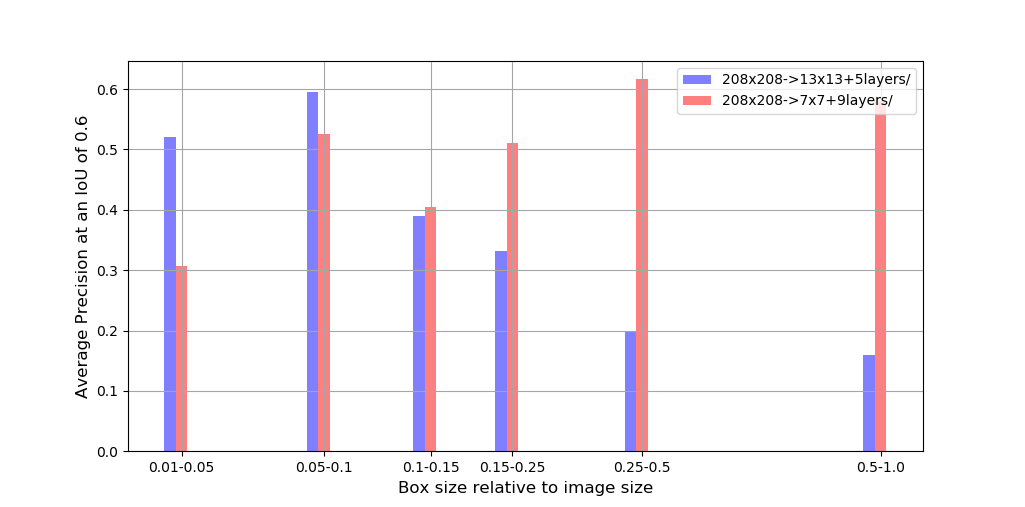
\includegraphics[width=\linewidth]{results_model}
	\caption{Average Precision for different box sizes on a test set of 1000 images.}
	\label{fig:model}
\end{figure}

\section{Next Steps}
\begin{itemize}
	\item Write it all down.
	\item Add prediction layers at multiple scales
	\item Investigate performance in terms of occlusion/angle
	\item Remove/Reduce occlusions from the dataset and repeat experiments. We could use the drone model we created for testing the filters to simulate the flight of a real drone and record the images.

\end{itemize}


\end{document}\grid
